
\documentclass{report}
\usepackage{graphicx} 
\usepackage[top=0.4in, bottom=.5in, left=0.8in, right=0.8in]{geometry}

\usepackage{subcaption}
\usepackage{amsmath}
\usepackage{amssymb}
\usepackage{multicol}
\usepackage{xcolor}
\usepackage{hyperref}

\newtheorem{theorem}{Teorema}
\newtheorem{definition}{Definición}



\setlength{\parindent}{0pt}

\begin{document}

\begin{center}

\textbf{}\\
\vspace{10cm}

\vspace{.2cm}
\textbf{Tratado de física de materiales}\\
\vspace{.2cm}
\textbf{Jesús Moral Aranda}\\
\vspace{.2cm}
\today
\end{center}
\newpage
\tableofcontents


\newpage
\chapter{Introducción}
\newpage
\chapter{Grupos de simetría en solidos cristalinos}
\section{Introducción}
Los átomos de un sólido que se acomodan formando estructuras periódicas, simétricas y ordenadas en el espacio, pueden ser modelizados mediante grupos de simetría. De manera que determinar el grupo de simetría de un arreglo de átomos permite capturar la información sobre las posiciones de los átomos en una red y determinar sus propiedades en función de las posiciones de los constituyentes de la red.\\

Una operación de simetría es una transformación del espacio afín  $\mathbb{R}^3$ que preserva distancias y ángulos que deja el patrón del cristal inalterado. La simetría del patrón del cristal es entonces entendido como la colección de operaciones de simetría del patrón.\\

- Si se aplican dos operaciones de simetría sucesivamente, el patrón queda inalterado. Por tanto la composición de operaciones de simetría es de nuevo una operación de simetría.\\

- Toda operación de simetría tiene su operación de simetría inversa.\\

Estas observaciones muestran que el conjunto de operaciones de simetría que compatibles con la estructura de la red, respecto a la composición de operaciones de simetría, tiene estructura de grupo.\\





\section{Introducción a grupos}

\subsection{Grupos}

\begin{definition}
 Un grupo es un conjunto \( G \) provisto de una ley de composición interna:

\[
G \times G \to G
\]

\[
(g,h) \mapsto gh
\]

con las siguientes propiedades:

\begin{enumerate}
    \item \textit{Asociatividad:}
    \[
    g(hk) = (gh)k, \quad \forall g,h,k \in G.
    \]
    
    \item \textit{Existencia del elemento neutro:}
    \[
    \exists e \in G \quad eg = ge = g, \quad \forall g \in G.
    \]
    
    \item \textit{Existencia de elementos inversos:}
    \[
    \forall g \in G, \quad \exists g^{-1} \in G  g^{-1} g = gg^{-1} = e.
    \]
  \end{enumerate}  

\end{definition}




\begin{definition}
Un grupo $G=\lbrace g_1,g_2,...,g_n\rbrace$ es \textbf{finito} si $|G|=n,\quad n<\infty$. De lo contrario se dice que es infinito.\\
\end{definition}


\begin{definition}
 El orden de \( g \), denotado por \( |g| \), es el menor entero positivo \( n \) tal que:
\[
g^n = e
\]
 Si no existe tal entero \( n \), decimos que \( g \) tiene orden infinito.
\end{definition}














\textit{Notación.} Si \( k \) es un entero no negativo y \( g \in G \) escribiremos

\[
g^k = \underbrace{g \cdots g}_{k \text{ factores}}, \quad 
g^{-k} = \underbrace{g^{-1} \cdots g^{-1}}_{k \text{ factores}},
\]

siendo \( g^0 \equiv e \). Nótese que esta notación no es ambigua, debido a la asociatividad del producto de un número arbitrario de elementos. Con la notación anterior, para todo \( i, j \in \mathbb{Z} \) se verifica:
\[
g^i g^j = g^{i+j}
\]

Alternativamente, cuando la ley de composición interna sea una suma ($+:G\times G \rightarrow G$, +(a,b)=a+b) se puede usar la notación aditiva. Esto es, las asociatividad se expresa como $(a+b)+c=a+(b+c)$, el elemento inverso de g como -g y elemento neutro e, como g+e=e+g=g. Además en esta notación, g+g+g=3g, en vez de $g^3$.\\

\vspace{.5cm}
\textit{Ejemplo: }El grupo puntual de simetría $6=\{1,2,3^+,3^-,6^+,6^-\}$. Donde el elemento n es una rotación de $\frac{2\pi}{n}$, n $\in$ $\{1,2,3,6 \}$. El 2=$2^+=2^-$ es su propio inverso, donde '$^+$' y '$^-$', indica sentidos de rotación horario y antihorario respectivamente. Las rotaciones son aplicaciones $f:\mathbb{R}^2\rightarrow \mathbb{R}^2$ o $f:\mathbb{R}^3\rightarrow \mathbb{R}^3$ , que son elementos clave de los grupos de simetría.




\begin{figure}[h!]
    \centering
    \begin{subfigure}{0.24\textwidth}
        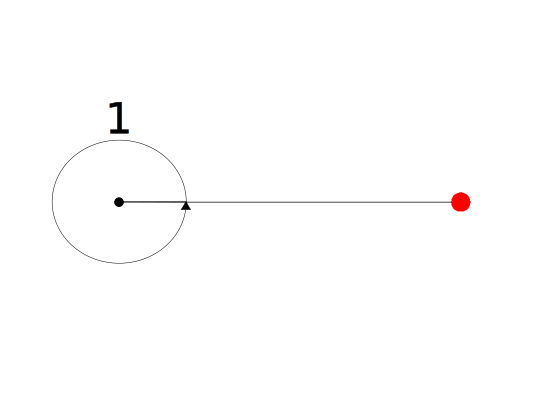
\includegraphics[width=\linewidth]{matlab/R_0.png}
        \caption{$1= \lbrace 1\rbrace$}
    \end{subfigure}
    \begin{subfigure}{0.24\textwidth}
        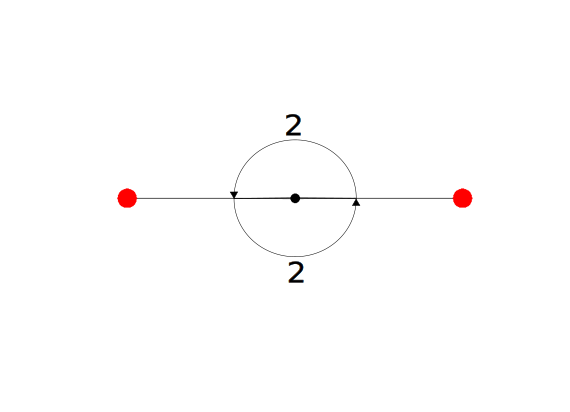
\includegraphics[width=\linewidth]{matlab/R_1.png}
        \caption{$ 2= \lbrace 1,2\rbrace$}
    \end{subfigure}
    \begin{subfigure}{0.24\textwidth}
        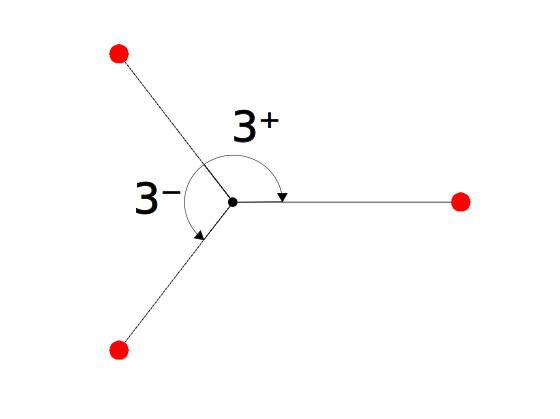
\includegraphics[width=\linewidth]{matlab/R_3b.png}
        \caption{$ 3= \lbrace 1, 3^+, 3^- \rbrace$}
    \end{subfigure}
    \begin{subfigure}{0.24\textwidth}
        \includegraphics[width=\linewidth]{matlab/R_4.png}
        \caption{$ 4= \lbrace 1, 2, 4^+, 4^- \rbrace$}
    \end{subfigure}

    \begin{subfigure}{0.24\textwidth}
        \includegraphics[width=.9\linewidth]{matlab/R_5.png}
        \caption{}$ 5= \lbrace 1, 5^+, 5^{++}, 5^-, 5^{--} \rbrace$
    \end{subfigure}
    \begin{subfigure}{0.24\textwidth}
    \fbox{
    \begin{minipage}{.9\linewidth}
        \centering
        \includegraphics[width=.9\linewidth]{matlab/R_6.png}
        \caption{}$ 6= \lbrace 1, 2, 3^+, 3^-, 6^+, 6^- \rbrace$
    \end{minipage}
}
    \end{subfigure}
    \begin{subfigure}{0.24\textwidth}
        \includegraphics[width=.9\linewidth]{matlab/R_7.png}
        \caption{}
        \tiny{  $ 7=\lbrace 1, 7^+, 7^{+2}, 7^{+3}, 7^-, 7^{-2}, 7^{-3} \rbrace $}
    \end{subfigure}
    \begin{subfigure}{0.24\textwidth}
        \includegraphics[width=.9\linewidth]{matlab/R_8.png}
        \caption{}$8=\lbrace 1, 2, 4^+, 4^-, 8^+, 8^- \rbrace$
    \end{subfigure}

    \caption{Grupos de rotaciones para ángulos de $2\pi$, $\pi$, 2$\pi$/3, $\pi$/2, 2$\pi$/5, $\pi$/3, 2$\pi$/7, $\pi$/4 }
\end{figure}

\hfill $\square$


\vspace{.5cm}
\subsection{Subgrupos}
\begin{definition}
Un \textit{subgrupo} $H$ de un grupo $G$,denotado como H $\leq$ G, es un subconjunto $H \subset G$ que es un grupo con el producto heredado de $G$. 
\end{definition}
\vspace{.2cm}

\begin{definition}
 Para cualquier $g\in G$
\[\langle g \rangle =\lbrace \; g^k \quad \vert \quad k\in \mathbb{Z} \; \rbrace \]\\

\end{definition}

Si $G=\{g_1,...,g_n\}$  es finito,la secuencia infinita $\{g^{0},g^1,...,g^n,....,g^m \}$,  necesariamente tiene al menos dos elementos tales que $g^{n}=g^j$ $0\leq j <n$. Más esquemáticamente nos podemos convencer de esto, al notar que es imposible una biyección entre ambos conjuntos:\\

\centering
\begin{tabular}{c c c c c c}

$\{g_1$ & ... & $g_n \}$ & &  &  \\ 
 
$\uparrow$ & $\uparrow$ & $\uparrow$ & $\hspace{-.4cm}\nwarrow$ & $\hspace{-.4cm}\nwarrow$ &  \\ 

$\{g^{0}$ & ... & $g^n$ & ... & $g^m$ & $\}$ \\ 

\end{tabular}\\
\raggedright
\vspace{.5cm}
De \( g^n = g^j \) con \( 0 \leq j < n \), se sigue que \( g^{n-j} = e = g^0 \). Por tanto, \( j = 0 \) y así \( g^n = e \).
Esto quiere decir que si G es finito, puedes coger cualquier elemento de este y el orden del elemento también es finito.\\
\vspace{.2cm}
Además, los elementos \( g^k \), para \( k = 1, \dots, n-1 \), son todos distintos, ya que cada \( g^k \) está en correspondencia uno a uno con los elementos de un subconjunto de \( G \), y \( k = n \) es la primera potencia que se repite. Más específicamente, se cumple que:

\[
\langle g^k \rangle = \{ e, g^1, \dots, g^{k-1} \} = H \leq G
\]
\[
g^i = g^j \quad \Leftrightarrow \quad i \equiv j \pmod{n} \quad \Leftrightarrow \quad i - j \equiv 0 \pmod{n}.
\]



\subsection{Grupos cíclicos}


\begin{definition}
Un grupo se denomina grupo ciclico de orden n, $C_n$ si:
\[
C_n =\lbrace e,g,g^2,g^3,...g^{k-1} \rbrace  \qquad \text{con el producto} \quad \forall i,j\quad g^i g^j=g^{i+j \; mod \; j}
\]
\end{definition}

Por tanto $\forall g\in G , \langle g\rangle $ es subgrupo cíclico de G. Si además se cumple que $\langle g\rangle$=G, entonces G es generado por un solo elemento y G es grupo cíclico. \\
\vspace{.2cm}
Los grupos cíclicos poseen importantes propiedades que facilitan el análisis de los mismos. Si G es un grupo cíclico de orden n entonces:





\begin{enumerate}
\item 
para cada divisor \( d \) de \( n \), existe exactamente un subgrupo de orden \( d \), dado por:
\[
H = \langle g^{n/d} \rangle.
\]

Esto significa que todos los subgrupos de \( G \) son también cíclicos.

\item  el orden de cualquier elemento \( g^k \) está dado por:
\[
|g^k| = \frac{n}{\gcd(k, n)}.
\]
Por lo tanto, el orden de cualquier elemento divide al orden del grupo.


\end{enumerate}



\vspace{.5cm}








\textit{Ejemplo:} El grupo puntual $6mm=\{1,m_{12},m_{21},m_{1-1},m_{11},m_{10},m_{01},2,3^+,3^-,6^+,6^-\}$, además de rotaciones contiene reflexiones, otro tipo de operación de simetría típico de los grupos puntuales. Los productos entre operaciones de simetría se pueden organizar como en la tabla \ref{raiza}.\\

\vspace{.2cm}

Además a cada operación de simetría le podemos asociar un elemento de simetría, que es un elemento geométrico asociado con una operación de simetría. Como se muestra en la figura \ref{6mm}. \\


\vspace{.2cm}


\begin{figure}[h!]
\centering
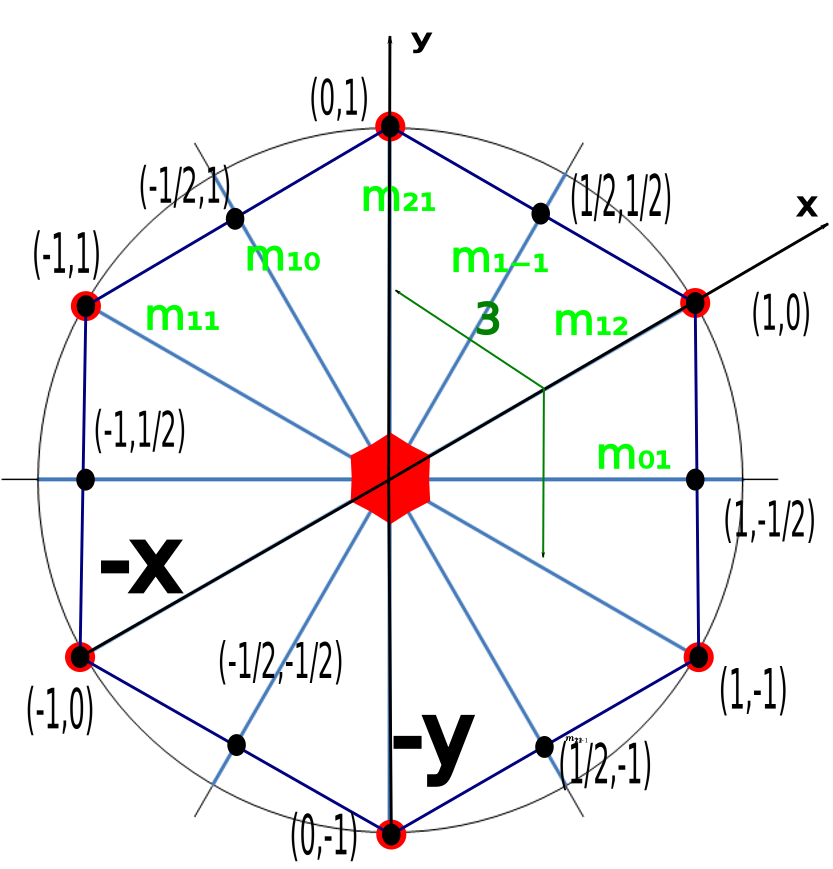
\includegraphics[width=.5\linewidth]{matlab/6mm.png}
\caption{Elementos de simetría de 6mm}
\label{6mm} 
\end{figure}



\begin{table}[h!]
\centering

   \[
\begin{array}{|c|c|c|c|c|c|c|c|c|c|c|c|c|c|}
\hline
6mm & & 1    & 2    & 3^+  & 3^-  & 6^+  & 6^-  & m_{12} & m_{21} & m_{1-1} & m_{11} & m_{10} & m_{01}\\
\hline
\vspace{-.2cm}
 & &     &     &   &  &  &   &  &  &  &  &  & \\
\hline
1 & & 1    & 2    & 3^+  & 3^-  & 6^+  & 6^-  & m_{12} & m_{21} & m_{1-1} & m_{11} & m_{10} & m_{01}\\
\hline
2 & & 2    & 1    & 6^-  & 6^+  & 3^-  & 3^+  & m_{10} & m_{01} & m_{11} & m_{1-1} & m_{12} & m_{21}\\
\hline
3^+& & 3^+  & 6^-  & 3^-  & 1    & 2    & 6^+  & m_{21} & m_{11} & m_{10} & m_{12} & m_{01} & m_{1-1}\\
\hline
3^-& & 3^-  & 6^+  & 1    & 3^+  & 6^-  & 2    & m_{11} & m_{12} & m_{01} & m_{21} & m_{1-1} & m_{10}\\
\hline
6^+& & 6^+  & 3^-  & 2    & 6^-  & 3^+  & 1    & m_{1-1} & m_{10} & m_{21} & m_{01} & m_{11} & m_{12}\\
\hline
6^-& & 6^-  & 3^+  & 6^+  & 2    & 1    & 3^-  & m_{01} & m_{1-1} & m_{12} & m_{10} & m_{21} & m_{11}\\
\hline
m_{12}& & m_{12} & m_{10} & m_{11} & m_{21} & m_{01} & m_{1-1} & 1    & 3^-  & 6^-  & 3^+   & 2  & 6^+\\
\hline
m_{21}& & m_{21} & m_{01} & m_{12} & m_{11} & m_{1-1} & m_{10} & 3^+  & 1    & 6^+  & 3^-  & 6^-    & 2\\
\hline
m_{1-1}& & m_{1-1} & m_{11} & m_{01} & m_{10} & m_{12} & m_{21}& 6^+  & 6^-  & 1    & 2  & 3^- & 3^+\\
\hline
m_{11}& & m_{11} & m_{1-1} & m_{21} & m_{12} & m_{10} & m_{01}  & 3^-    & 3^+  & 2  & 1    & 6^+  & 6^-\\
\hline
m_{10}& & m_{10} & m_{12} & m_{1-1} & m_{01} & m_{21} & m_{11} & 2 & 6^+   & 3^+  & 6^-  & 1    & 3^-\\
\hline
m_{01} & & m_{01} & m_{21} & m_{10} & m_{1-1} & m_{11} & m_{12}  & 6^-  & 2  & 3^-    & 6^+ & 3^+  & 1\\
\hline
\end{array}
\]

\caption{Tabla de multiplicación de 6mm}
\label{raiza}
\end{table}
\raggedright



La relación grupo-subgrupo para 6mm se puede representar gráficamente como en la figura \ref{raizatq}. Se puede observar que los ordenes de los subgrupos son los divisores del orden del grupo. \\

\vspace{.2cm}


El grupo 6mm no es cíclico, uno se puede convencer de esto al notar que el producto de rotaciones son rotaciones, pero no así el producto de reflexiones. De modo que necesitas al menos de una rotación y una reflexión para generar todo el grupo. Sin embargo los subgrupos 6, 3, 2 de rotaciones , al igual que m, sí son cíclicos.

.\\
\vspace{.2cm}







\newpage


\begin{figure}[h!]
\centering
\includegraphics[width=.7\linewidth]{matlab/6mmsg.png}
\end{figure}


\begin{multicols}{2}



Los subgrupos de 6mm son:


\[\textcolor{blue}{  6mm}=
\{1, 2, 3^+, 3^-, 6^+, 6^-, m_{12}, m_{21}, m_{1-1}, m_{11}, m_{10}, m_{01} \}
\]
\[\textcolor{blue}{6}=
\{1, 6^+, 3^+, 2, 3^-, 6^-\}  
\]


\[\textcolor{blue}{
3m \equiv 3m_1, 3m_2}
\]
\[
3m_2 = \{1, 3^+, 3^-, m_{12}, m_{21}, m_{11}\}
\]
\[
3m_1 = \{1, 3^+, 3^-, m_{1-1}, m_{10}, m_{01}\}
\]
\columnbreak

\[\textcolor{blue}{
mm2 \equiv mm2_1, mm2_2, mm2_3}
\]

\[
mm2_1 = \{1, 2, m_{1-1}, m_{11}\}
\]
\[
mm2_2 = \{1, 2, m_{10}, m_{12}\}
\]
\[
mm2_3 = \{1, 2, m_{21}, m_{01}\}
\]

\[\textcolor{blue}{  
m} \equiv \{1, m_{12}\}, \{1, m_{21}\}, \{1, m_{11}\}, \{1, m_{1-1}\}, \{1, m_{10}\}, \{1, m_{01}\}
\]
\[\textcolor{blue}{ 3}=
\{1, 3^+, 3^-\} 
\]
\[\textcolor{blue}{  2}=
\{1, 2\} 
\]
\[\textcolor{blue}{1}=
\{1\} 
\]


\end{multicols}
\newpage


\begin{figure}[h!]
\caption{Diagrama Grupo-Subgrupo de 6mm}
\label{raizatq}
\end{figure}








\hfill $\square$
















\subsection{Cosets. Teorema de Lagrange}
\begin{definition}
Si \( H \) es un subgrupo de un grupo \( G \), definimos el \textbf{coset} (por la izquierda) asociado a un elemento cualquiera \( a \in G \) como el conjunto
\[
aH \equiv \{ ah \mid h \in H \}.
\]
\end{definition}
El coset por la derecha \( Ha \) se define de forma análoga. Es inmediato probar que:

\begin{enumerate}
    \item \label{1} El coset \( aH \) coincide con \( H \) si y solo si \( a \in H \),
    \item Si \( a \notin H \), la unidad \( e \) no pertenece a \( aH \), de esto se sigue que el único coset de H que es subgrupo es el propio H.
    \item Si \( G \) es finito, \( H \) y \( aH \) tienen el mismo número de elementos para todo \( a \in G \), es decir:
\end{enumerate}
\[
|aH| = |H|.
\]
La propiedad fundamental de los cosets es la siguiente:\\
\vspace{.2cm}
\textbf{Proposición:}
Sea \( H \) subgrupo de un grupo \( G \), y sean \( a, b \) elementos de \( G \). Entonces los correspondientes cosets \( aH \), \( bH \), o son iguales, o son disjuntos.\\



\textit{Demostración.} En efecto, supongamos que \( aH \cap bH \neq \emptyset \), y sea \( g \in aH \cap bH \). Por definición de coset, existen dos elementos \( h_1, h_2 \in H \) tales que
\[
g = ah_1 = bh_2.
\]
Entonces los cosets \( aH \) y \( bH \) son iguales, ya que
\[
bH = a(h_1 h_2^{-1})H = aH
\]
en virtud de la primera propiedad \ref{1} de los cosets (nótese que \( h_1 h_2^{-1} \in H \), al ser este conjunto un subgrupo). 
\[\hspace{18cm}\square\]


En virtud de la proposición anterior, si \( H \) es un subgrupo cualquiera de un grupo (finito o infinito) \( G \) entonces \( G \) es una \textit{unión disjunta de cosets} asociados al subgrupo \( H \) (es decir los cosets forman una partición de G). Si \( G \) (y, por tanto, \( H \)) es finito, esto quiere decir que existen \( m \) elementos \( a_1, \dots, a_m \in G \) tales que \( a_i H \cap a_j H = \emptyset \) para todo \( i \neq j \) y

\[
G = \bigcup_{i=1}^{m} a_i H.
\]

Al ser los cosets \( a_i H \) disjuntos y \( |a_i H| = |H| \), de la ecuación anterior se sigue que

\[
|G| = m |H|.
\]

Esto demuestra el siguiente teorema, probado por vez primera por Lagrange:

\begin{theorem}
Si \( G \) es un grupo finito y \( H \) es un subgrupo de \( G \), el orden de \( H \) divide al de \( G \).
\end{theorem}













\begin{definition}
Si \( G \) es un grupo finito y \( H \) es un subgrupo de \( G \), el \textbf{índice} de \( H \),i(H), es el número de cosets de \( H \), es decir (en virtud de la demostración del teorema de Lagrange) el cociente \( |G| / |H| \).
\label{8}
\end{definition}



De este teorema se sigue, que un grupo finito \( G \) de orden primo  n  es equivalente (es decir, isomorfo; cf. secciones siguientes) a \( C_n \).Por que del teorema de Lagrange se sigue que \( G \) no posee subgrupos propios (es decir, distintos de \( \{e\} \) y del propio \( G \)).  Si \( |G| > 1 \) y \( g \neq e \) es un elemento cualquiera de \( G \), el conjunto

\[
\{ e, g, \dots, g^{m-1} \}, \quad \text{con} \quad m = o(G),
\]

es un subgrupo de \( G \) de orden \( m > 1 \), de donde se sigue que \( m = n \). Por tanto

\[
G = \{ e, g, \dots, g^{n-1} \}
\]

es equivalente a \( C_n \), al ser \( g^n = e \). En el ejemplo anterior los subgrupos de orden 2 y 3 eran cíclicos.




\vspace{.2cm}




Para obtener la descomposición en cosets, se comienza eligiendo $\mathcal{H}$ como el primer coset (con representante $e$). A continuación, se selecciona un elemento $g_2 \in \mathcal{G}$ con $g_2 \notin \mathcal{H}$ como representante del segundo coset $g_2\mathcal{H}$. Para el tercer coset, se requiere un elemento $g_3 \in \mathcal{G}$ con $g_3 \notin \mathcal{H}$ y $g_3 \notin g_2\mathcal{H}$. Si en cierta etapa los cosets $\mathcal{H}, g_2\mathcal{H}, \dots, g_m\mathcal{H}$ han sido definidos pero no agotan $\mathcal{G}$, se elige un elemento $g_{m+1}$ que no está contenido en la unión $\mathcal{H} \cup g_2\mathcal{H} \cup \dots \cup g_m\mathcal{H}$ como representante del siguiente coset.\\
\vspace{.5cm}

\textit{Ejemplo:} 


\[G=\textcolor{red}{6mm}=
\{1, 2, 3^+, 3^-, 6^+, 6^-, m_{12}, m_{21}, m_{1-1}, m_{11}, m_{10}, m_{01} \}
\]
\hrulefill
\raggedright




\[ H=\textcolor{blue}{6}=
\{1, 6^+, 3^+, 2, 3^-, 6^-\} \qquad \qquad 1\textcolor{blue}{6} \quad =
\{1, 6^+, 3^+, 2, 3^-, 6^-\} 
\quad 
 m_{12}\textcolor{blue}{6}=\{m_{12}, m_{21}, m_{1-1}, m_{11}, m_{10}, m_{01} \}
\]


\[\textcolor{red}{6mm}=\textcolor{blue}{6}\cup m\textcolor{blue}{6}\]
\[\textcolor{red}{6}=\textcolor{blue}{3}\cup 2\textcolor{blue}{3}\]
\[\textcolor{red}{6}=\textcolor{blue}{2}\cup 3\textcolor{blue}{2}\]
\hrulefill
\vspace{.5cm}

\[H=\textcolor{blue}{
3m \equiv}=\{1, 3^+, 3^-, m_{12}, m_{21}, m_{11}\}
\qquad \qquad 1\textcolor{blue}{
3m} \quad 2\textcolor{blue}{
3m}=\{2,6^+,6^-,m_{1-1},m_{10},m_{01} \}
\]

\[\textcolor{red}{6mm}=\textcolor{blue}{3m}\cup 2\textcolor{blue}{3m}\]


\hrulefill
\vspace{.5cm}

\[H=\textcolor{blue}{
mm2}=\{1,2,m_{-},m_{|}\} 
\qquad \qquad 3^+\textcolor{blue}{
mm2}=\{3^+,6^-,m_{-},m_{|}\} 
\quad 
3^-\textcolor{blue}{
mm2}=\{3^-,6^+,m_{-},m_{|}\}  
  \]
  
  \[\textcolor{red}{6mm}=\textcolor{blue}{mm2}\cup 3^+\textcolor{blue}{mm2}\cup 3^-\textcolor{blue}{mm2}\]





\newpage
\subsection{Relación de conjugación. Subgrupos normales y grupo cociente}

\begin{definition}
Dados dos elementos \( a, b \) de un grupo \( G \), se dice que \( b \) está \textbf{conjugado} con \( a \) si \( b \) es la imagen de \( a \) bajo la conjugación por algún elemento del grupo, es decir si

\[
b = g a g^{-1}
\]

para algún \( g \in G \). Escribiremos en tal caso \( b \sim a \).

\end{definition}



 Es fácil ver que la relación \( \sim \) definida de este modo es una \textbf{relación de equivalencia}, es decir \(\forall a, b, c \in G\) se cumple:

\begin{enumerate}
    \item \( a \sim a \) \quad (reflexividad)
    \item \( b \sim a \iff a \sim b \) \quad (simetría)
    \item \( a \sim b, \quad b \sim c \implies a \sim c \) \quad (transitividad)
\end{enumerate}

\begin{definition}
La clase de conjugación de \( a \in G \) es la clase de equivalencia bajo la conjugación a la que pertenece dicho elemento, es decir el conjunto \([a]\) dado por:

\[
[a] = \{ g a g^{-1} \mid g \in G \}.
\]
\end{definition}
Nótese que, por definición:

\[
b \in [a] \iff b \sim a.
\qquad
b \in [a] \leftrightarrow \quad [a]=[b]\]


Esto sugiere que las clases de conjugación también producen una partición de G.


\begin{theorem}


Un grupo cualquiera \( G \) es la unión disjunta de sus clases de conjugación. En otras palabras,

\[[a] \cap [b] \neq \emptyset \quad \Longrightarrow \quad [a] = [b].\]

\end{theorem}
\textit{Demostración.} En efecto,

\[
c \in [a] \cap [b] \quad \Longrightarrow \quad c \sim a, \; c \sim b \quad \Longleftrightarrow \quad b \sim c, \; c \sim a \quad \Longrightarrow \quad b \sim a \quad \Longleftrightarrow \quad [a] = [b].
\]

\hfill \(\Box\)


Como veremos un aspecto importante de los elementos conjugados en los grupos de simetría , es que comparten muchas propiedades, como el orden o el tipo de operación de simetría. Como consecuencia, las operaciones de simetría conjugadas tienen el mismo tipo de elementos geométricos.\\
\vspace{.5cm}


\textit{Ejemplo:}
Las clases de conjugación permite distinguir los tipos de rotaciones y de reflexiones. Las rotaciones en cambio si se separan en función del ángulo de rotación, no distinguiendo el sentido de la rotación.\\
\vspace{.2cm} 
 Pero las reflexiones solo se distinguen entre ellas por como están conjugadas con las demás reflexiones. Siendo que si un eje de reflexión esta relacionado con otro por una rotación de $6^\pm$, entonces estos dos son equivalentes o conjugados.
 Por ejemplo en $[m_{12}]$,  $ 6^+ m_{12}6^-=m_{21}\quad \rightarrow m_{12}\sim m_{21}$. Lo mismo para $[m_{1-1}]$. 
\[
 \textcolor{red}{[1]} = \{1\}
\quad
 \textcolor{red}{ [2]} = \{2\}
\quad
 \textcolor{red}{[3]} = \{3^+, 3^-\}
\quad
  \textcolor{red}{[6^+]} = \{6^+, 6^-\}
\quad
  \textcolor{red}{[m_{12}]} = \{m_{12}, m_{21}, m_{11} \}
\quad
  \textcolor{red}{[m_{10}]} = \{m_{1-1}, m_{10}, m_{01} \}
\]


\hfill $\square$\\


\subsection{Subgrupos normales}
\begin{definition}
 Un subgrupo H de un grupo G es normal (H $\triangleleft$ G) si:
\[
g H g^{-1} = H , \quad \forall g \in G.
\]

Equivalentemente, \( H \) es un subgrupo normal si y solo si
\[
gH = Hg , \quad \forall g \in G.
\]
\end{definition}


La expresión \( g H g^{-1} \) denota el conjunto de todos los elementos de la forma \( ghg^{-1} \) con \( h \in H \), es decir:
\[
g H g^{-1} = \{ ghg^{-1} \mid h \in H \}.
\]
Si se cumple que \( g H g^{-1} = H \) para todo \( g \in G \), significa que \( H \) es invariante bajo conjugación, lo que caracteriza a los subgrupos normales.\\

\vspace{.2cm}
Propiedades de los subgrupos normales:
\begin{enumerate}
\item
Si \( \mathcal{G} \) y \( \mathcal{H} \) están generados por un conjunto de elementos, entonces basta con verificar la condición de normalidad solo para los generadores.  
Es decir, si verificamos que:
\[
g_i h g_i^{-1} \in \mathcal{H}
\]
para cada generador \( g_i \) de \( \mathcal{G} \) y  de \( \mathcal{H} \), entonces la propiedad se extiende a todos los elementos de \( \mathcal{G} \).

\item \textit{Un subgrupo \( H \) de un grupo \( G \) es normal si y solo si}

\[
h \in H \quad \Longrightarrow \quad [h] \in H.
\]

En otras palabras, un subgrupo \( H \subset G \) es normal si y solo si \( H \) \textit{es la unión de clases de conjugación completas de} \( G \). 



\end{enumerate}























\subsection{Grupo cociente}

Si \( H \) es un subgrupo de un grupo \( G \), parece natural definir un producto entre los cosets (por la izquierda) de \( H \) mediante la fórmula

\[
aH \cdot bH = (ab)H.
\]



¿Es esta definición correcta? Para que lo sea debemos comprobar que depende exclusivamente de los cosets \( aH \) y \( bH \), y no de los elementos \( a \) y \( b \) que se han seleccionado implícitamente para describir dichos cosets. En otras palabras, debemos comprobar que

\[
aH = a'H , \quad bH = b'H \implies aH \cdot bH = a'H \cdot b'H.
\]

o equivalentemente:

\[
aH = a'H , \quad bH = b'H \implies (ab)H = (a'b')H.
\]

Para ello, nótese en primer lugar que

\[
aH = a'H \iff a' = ah_1 , \quad bH = b'H \iff b' = bh_2 \quad \text{con } h_1, h_2 \in H.
\]

Por tanto,

\[
(a'b')H = (ah_1 bh_2)H,
\]

que, en general es distinto de \( (ab)H \).\\

\vspace{.2cm}


Por lo que acabamos de ver, la condición necesaria y suficiente para que el producto “natural” de cosets  esté bien definido es que se cumpla la condición, es decir:

\[
(a h_1 b h_2)H = (ab)H \iff a h_1 b h_2 \in abH
\quad
\iff b^{-1} h_1 b h_2 \in H, \quad \forall b \in G, \quad \forall h_1, h_2 \in H.
\]

\begin{equation} \label{eq:condicion_normal}
b^{-1} h_1 b h_2 \in H, \quad \forall b \in G, \quad \forall h_1, h_2 \in H.
\end{equation}

Esta condición se cumple automáticamente si el subgrupo \( H \) es normal; de hecho, (\ref{eq:condicion_normal}) es equivalente al carácter normal de \( H \), como se deduce sin más que tomar \( h_2 = e \). Por tanto, el producto de cosets de un subgrupo \( H \) está bien definido si y solo si \( H \) es normal.\\
\vspace{.2cm}

Supongamos, en vista de lo anterior, que el subgrupo \( H \) es \emph{normal}, y definamos el producto de cosets de \( H \) por $aH \cdot bH = (ab)H$. Es fácil comprobar entonces que el conjunto:

\[
G/H = \{ aH \mid a \in G \}
\]

cuyos elementos son los cosets (por la izquierda) de \( H \) es un grupo respecto del producto que acabamos de definir. En efecto:


\begin{enumerate}
    \item La propiedad asociativa es consecuencia de la asociatividad del producto en \( H \):

    \[
    (aH)(bH) \cdot cH \equiv (aH)((bc)H) = (a(bc))H = ((ab)c)H = ((ab)H) \cdot cH
\quad 
    \equiv (aH \cdot bH)(cH).
    \]

    \item La unidad de \( G/H \) es el subgrupo \( H \), ya que

    \[
    H \cdot aH \equiv eH \cdot aH \equiv (ea)H = aH, \quad \forall a \in G.
    \]

    \item \( (aH)^{-1} = a^{-1} H \).
\end{enumerate}
\vspace{.2cm}
Teniendo esto ya en consideración podemos definir el grupo cociente:\\
\vspace{.2cm}

\begin{definition}
 Si \( H \) es un subgrupo normal de un grupo \( G \), el \emph{grupo cociente} de \( G \) por \( H \) es el conjunto \( G/H \) de los cosets (por la izquierda) de \( H \) con el producto $aH \cdot bH = (ab)H$.
\end{definition}




\begin{itemize}
    \item Si \( G \) es un grupo finito, por el teorema de Lagrange \( G/H \) es un grupo finito de orden:
    \[
    |G/H| = \frac{|G|}{|H|}
    \]
\end{itemize}
\vspace{.5cm}

\textit{Ejemplo:} Grupos Cociente de \(6mm\). Lo primero es darse cuenta de que solo podemos dar los grupos cociente de subgrupos normales. Por ejemplo de 6 y 3.







\begin{multicols}{2}
\subsection*{\( \textcolor{red}{6mm} / \textcolor{blue}{6} \cong \mathbb{Z}_{2} \)}
\[
\textcolor{red}{6mm} / \textcolor{blue}{6} = \{ \textcolor{blue}{6}, m_{12}\textcolor{blue}{6} \},
\]
\[
\textcolor{blue}{6} = \{1, 6^+, 3^+, 2, 3^-, 6^-\}, \quad m_{12}\textcolor{blue}{6} = \{m_{12}, m_{21}, m_{1-1}, m_{11}, m_{10}, m_{01} \}.
\]
\columnbreak
\[
\begin{array}{c|cc}
\cdot & \textcolor{blue}{6} & m_{12}\textcolor{blue}{6}\\ \hline
\textcolor{blue}{6} & \textcolor{blue}{6} & m_{12}\textcolor{blue}{6}\\
m_{12}\textcolor{blue}{6} & m_{12}\textcolor{blue}{6} & \textcolor{blue}{6}
\end{array}
\]
\end{multicols}

\begin{multicols}{2}
\subsection*{\( \textcolor{red}{6mm} / \textcolor{blue}{3} \cong V_4 \)}
\[
\textcolor{red}{6mm} / \textcolor{blue}{3} = \{ \textcolor{blue}{3}, 2\textcolor{blue}{3}, m_{12}\textcolor{blue}{3}, m_{1-1}\textcolor{blue}{3} \},
\]
\[
\textcolor{blue}{3} = \{1, 3^+, 3^-\}, \quad 2\textcolor{blue}{3} = \{2, 6^+, 6^-\},
\]
\[
 m_{12}\textcolor{blue}{3} = \{m_{12}, m_{11}, m_{21}\}, \quad m_{1-1}\textcolor{blue}{3} = \{m_{1-1}, m_{10}, m_{01}\}.
\]
\columnbreak
\[
\begin{array}{c|cccc}
\cdot & \textcolor{blue}{3} & 2\textcolor{blue}{3} & m_{12}\textcolor{blue}{3} & m_{1-1}\textcolor{blue}{3}\\ \hline
\textcolor{blue}{3} & \textcolor{blue}{3} & 2\textcolor{blue}{3} & m_{12}\textcolor{blue}{3} & m_{1-1}\textcolor{blue}{3}\\
2\textcolor{blue}{3} & 2\textcolor{blue}{3} & \textcolor{blue}{3} & m_{1-1}\textcolor{blue}{3} & m_{12}\textcolor{blue}{3}\\
m_{12}\textcolor{blue}{3} & m_{12}\textcolor{blue}{3} & m_{1-1}\textcolor{blue}{3} & \textcolor{blue}{3} & 2\textcolor{blue}{3}\\
m_{1-1}\textcolor{blue}{3} & m_{1-1}\textcolor{blue}{3} & m_{12}\textcolor{blue}{3} & 2\textcolor{blue}{3} & \textcolor{blue}{3}
\end{array}
\]
\end{multicols}


\vspace{1cm}
\subsection{Homomorfismos}
\begin{definition}
 Un homomorfismo entre dos grupos \( G \) y \( G' \) es una aplicación \( \varphi: G \to G' \) que verifica

\[
\varphi(gh) = \varphi(g) \varphi(h), \quad \forall g,h \in G.
\]
\end{definition}
 Un isomorfismo es un homomorfismo biyectivo, y un automorfismo es un isomorfismo de un grupo \( G \) en sí mismo.

En otras palabras, un homomorfismo es una aplicación \( G \to G' \) que preserva el producto, y por tanto la estructura de grupo. En particular, dos grupos son isomorfos, $G \cong G'$, si son totalmente equivalentes desde el punto de vista de la teoría de grupos, constituyendo dos realizaciones distintas del mismo grupo abstracto, un cambio de etiquetas.\\

\vspace{.4cm}

\textbf{Proposición:} \textit{Sea} \( \varphi: G \to G' \) \textit{un homomorfismo. Entonces se verifica:}

\begin{enumerate}
    \item \( \varphi(e) = e' \), \textit{siendo} \( e' \) \textit{la unidad de} \( G' \).
    \item \( \varphi(g^{-1}) = \varphi(g)^{-1}, \quad \forall g \in G \).
\end{enumerate}



\textit{Demostración.}

1) Si \( g \in G \) se tiene
\[
\varphi(g) = \varphi(g e) = \varphi(g) \varphi(e) \quad \Longrightarrow \quad \varphi(e) = e'.
\]

2) Utilizando el apartado anterior se tiene
\[
\varphi(g) \varphi(g^{-1}) = \varphi(gg^{-1}) = \varphi(e) = e' 
\quad \Longrightarrow \quad \varphi(g^{-1}) = \varphi(g)^{-1}.
\]




\vspace{.4cm}





\subsection{Representaciones}
\begin{definition}
 Sea \( G \) un grupo, y \( V \) un espacio vectorial complejo de dimensión finita. Una representación lineal de \( G \) en el espacio vectorial \( V \) es un homomorfismo \( D: G \to \text{GL}(V) \). La dimensión de \( V \) como espacio vectorial se denomina dimensión de la representación \( D \). Una representación se dice fiel si es inyectiva.

\end{definition}

\begin{definition}
 Sea \( V \) un espacio vectorial (de dimensión finita o infinita, real o complejo), y definamos:

\[
GL(V) = \{ f: V \to V \mid f \text{ lineal e invertible} \}.
\]
\end{definition}


Nótese que, por las propiedades de los homomorfismos, si \( D \) es una representación de \( G \) entonces
\[
D(e) = I, \quad D(g^{-1}) = D(g)^{-1},
\]
siendo \( I: V \to V \) la aplicación identidad.







\begin{definition}
Una representación matricial de un grupo \( G \) es un \textit{homomorfismo} \( D : G \to \text{GL}(n, \mathbb{R}) \).

\medskip

Si \( V = \mathbb{R}^n \) se identifica normalmente \( \text{GL}(\mathbb{R}^n) \) con \( \text{GL}(n, \mathbb{R}) \), equiparando una aplicación lineal \( A : \mathbb{R}^n \to \mathbb{R}^n \) con su matriz en la base canónica de \( \mathbb{R}^n \). Mediante esta identificación, podemos considerar las representaciones matriciales como un caso particular de las lineales.\\

\[
\text{GL}(n, \mathbb{R}) = \left\{ A \in M_{n\times n}(\mathbb{R}) \mid A \text{ es invertible} \right\},
\]

\end{definition}

De modo que podemos asociar a las operaciones de simetría de los grupos puntuales y espaciales con matrices de la aplicación lineal.




\vspace{.4cm}

\textit{Ejemplo:}
Sea \( D: 6mm \to GL(3, \mathbb{R}) \) la representación matricial del grupo puntual \( 6mm \), asignamos a cada operación de simetría su correspondiente matriz:\\
\vspace{.4cm}
\small{
\[
\begin{array}{cccc}
D(1) = 
\begin{pmatrix} 
1 & 0 & 0 \\ 
0 & 1 & 0 \\ 
0 & 0 & 1 
\end{pmatrix},
&
D(3^+) = 
\begin{pmatrix} 
-1 & -1 & 0 \\ 
1 & 0 & 0 \\ 
0 & 0 & 1 
\end{pmatrix},
&
D(3^-) = 
\begin{pmatrix} 
0 & -1 & 0 \\ 
1 & 1 & 0 \\ 
0 & 0 & 1 
\end{pmatrix},
&
D(2) = 
\begin{pmatrix} 
-1 & 0 & 0 \\ 
0 & -1 & 0 \\ 
0 & 0 & 1 
\end{pmatrix},
\\[20pt]
D(6^+) = 
\begin{pmatrix} 
0 & -1 & 0 \\ 
1 & 0 & 0 \\ 
0 & 0 & 1 
\end{pmatrix},
&
D(6^-) = 
\begin{pmatrix} 
1 & 1 & 0 \\ 
-1 & 0 & 0 \\ 
0 & 0 & 1 
\end{pmatrix},
&
D(m_{110}) = 
\begin{pmatrix} 
-1 & 0 & 0 \\ 
0 & 1 & 0 \\ 
0 & 0 & 1 
\end{pmatrix},
&
D(m_{100}) = 
\begin{pmatrix} 
-1 & -1 & 0 \\ 
-1 & 0 & 0 \\ 
0 & 0 & 1 
\end{pmatrix},
\\[20pt]
D(m_{010}) = 
\begin{pmatrix} 
1 & 0 & 0 \\ 
0 & -1 & 0 \\ 
0 & 0 & 1 
\end{pmatrix},
&
D(m_{1-10}) = 
\begin{pmatrix} 
0 & 1 & 0 \\ 
1 & 0 & 0 \\ 
0 & 0 & 1 
\end{pmatrix},
&
D(m_{120}) = 
\begin{pmatrix} 
1 & 0 & 0 \\ 
0 & -1 & 0 \\ 
0 & 0 & 1 
\end{pmatrix},
&
D(m_{210}) = 
\begin{pmatrix} 
-1 & 1 & 0 \\ 
1 & 0 & 0 \\ 
0 & 0 & 1 
\end{pmatrix}.
\end{array}
\]
}
\hfill $\square$
\vspace{.4cm}
\subsection{Acciones de grupo sobre conjuntos}

\begin{definition}
\textbf{Definición.} Una \textit{acción de grupo} de un grupo \( G \) sobre un conjunto \( \Omega = \{ \omega \mid \omega \in \Omega \} \) asigna a cada par \( (g, \omega) \) un objeto \( \omega' = g(\omega) \) de \( \Omega \) tal que se cumplen las siguientes condiciones:

\begin{itemize}
    \item[(i)] Aplicar dos elementos \( g \) y \( g' \) del grupo consecutivamente tiene el mismo efecto que aplicar el producto \( g' g \), es decir, 
    \[
    g'(g(\omega)) = (g' g)(\omega).
    \]
    (Nótese que los elementos del grupo actúan \textit{desde la izquierda} sobre los objetos en \( \Omega \), por lo que en un producto de dos o más elementos del grupo, estos se aplican de derecha a izquierda).
    
    \item[(ii)] Aplicar el elemento identidad \( e \) de \( G \) no tiene efecto sobre \( \omega \), es decir,
    \[
    e(\omega) = \omega, \quad \forall \omega \in \Omega.
    \]
\end{itemize}

Se dice que el objeto \( \omega \) es \textit{movido} a \( g(\omega) \) por \( g \).

\end{definition}




\textbf{Definición.} Dos objetos \( \omega, \omega' \in \Omega \) pertenecen a la misma \textit{órbita} bajo \( G \) si existe \( g \in G \) tal que \( \omega' = g(\omega) \).

El conjunto 
\[
\mathcal{G}(\omega) := \{ g(\omega) \mid g \in G \}
\]
de todos los objetos en la órbita de \( \omega \) se llama la \textit{órbita de \( \omega \) bajo \( G \)}.\\
\vspace{.2cm}
El conjunto 
\[
S_G(\omega) := \{ g \in G \mid g(\omega) = \omega \}
\]
de los elementos del grupo que no mueven el objeto \( \omega \) es un subgrupo de \( G \) llamado el \textit{estabilizador} de \( \omega \) en \( G \).\\
\vspace{.2cm}



\vspace{.4cm}


\textit{Ejemplo:} Acción de \(6mm\) sobre los vertices de un hexágono, órbitas y estabilizadores.\\

\[
 \textcolor{red}{6mm}
\;=\;
\{\,1,\,2,\,3^+,\,3^-,\,6^+,\,6^-,\,m_{12},\,m_{21},\,m_{1-1},\,m_{11},\,m_{10},\,m_{01}\}
\]


\begin{figure}[h!]
\centering
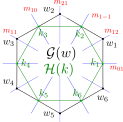
\includegraphics[width=.5\textwidth]{matlab/orbit.png} 
\caption{dos orbitas de 6mm}
\end{figure}













\medskip

-Acción sobre los vértices de un hexágono.\\

\vspace{.2cm}
Consideremos dos conjuntos de puntos distintos.
\[
\Omega \;=\; \{\omega_1,\,\omega_2,\,\omega_3,\,\omega_4,\,\omega_5,\,\omega_6\}.
\]
\[
\beta \;=\; \{k_1,\,k_2,\,k_3,\,k_4,\,k_5,\,k_6\}.
\]

Definimos una acción de grupo de 6mm sobre \(\Omega\) y $\beta$ haciendo que cada elemento de 6mm (rotación o reflexión) \emph{mueva} un vértice \(\omega_i\) a la posición correspondiente (por ejemplo, una rotación de 60º lleva \(\omega_1 \mapsto \omega_2\), \(\omega_2 \mapsto \omega_3\), etc., y una reflexión puede fijar un vértice y permutar los restantes).\\
\vspace{.2cm}
-Órbita de un vértice.\\
Tomemos un vértice concreto, por ejemplo \(\omega_1\). Dado que \(6mm\) contiene rotaciones que abarcan todos los vértices (60º, 120º, etc.), la \emph{órbita} de \(\omega_1\) es todo el conjunto de vértices:
\[
\mathcal{G}(\omega)
\;=\;
\{\omega_1,\,\omega_2,\,\omega_3,\,\omega_4,\,\omega_5,\,\omega_6\}.
\]
Lo mismo para 
\[
\mathcal{H}(k)
\;= \{k_1,\,k_2,\,k_3,\,k_4,\,k_5,\,k_6\}.
\]

\vspace{.2cm}

-Estabilizador de un vértice.\\
\vspace{.2cm}
En el caso de la orbita de w, los estabilizadores son:
\[
S_6mm(\omega)
=\{1,m_{12},m_{21},m_{11}\},
\]
En cambio para la orbita de k, los estabilizadores son los otros tipos de ejes
\[
S_6mm(k)
=\{1,m_{1-1},m_{01},m_{10}\},
\]
\hfill $\square$
\newpage

\section{Grupos puntuales cristalográficos}

Para determinar que el número de grupos puntuales compatibles con la periodicidad de una red son exactamente 32, podemos seguir la recomendación de Kant y Platón para el método de todo saber en general. Debemos satisfacer dos leyes trascendentales de la razón, la de homogeneidad y la de especificación. La primera nos manda que, atendiendo a las semejanzas de las cosas, concibamos clases, y que a su vez, unifiquemos estas en especies y las especies en géneros. En cambio la ley de espicificación exige que distingamos bien las especies unificadas en un concepto de género, guardándonos de dar cualquier salto\footnote{Arthur Schopenhauer, Sobre la cuádruple raíz del principio de razón suficiente, Capítulo 1: "El método".}.\\
\vspace{.2cm}

Del infinito número de grupos puntuales que se pueden  generar a partir de las rotaciones de $\frac{2\pi}{n}, n\in \mathbb{Z}^+$. Cabe restringuir  las rotaciones a $\{1,2,3,4,6\}$. 
La restricción a estas rotaciones es debido a la restricción cristalográfica, es decir, al problema de teselar el espacio:\\
\vspace{.2cm}



Sea $R\in SO(3)$ la representación matricial de la rotación de ángulo $\frac{2\pi}{n}, n\in \mathbb{Z}^+$. Al ser una transformación ortogonal $R_{ik}R_{jk}=\delta_{ij}$ y eligiendo de manera conveniente los ejes, se sigue que las matrices de rotación tienen la forma:


\[
R_{ij} =
\begin{bmatrix}
\cos\theta & -\sin\theta & 0 \\ 
\sin\theta & \cos\theta & 0 \\ 
0 & 0 & 1
\end{bmatrix}
\]

La traza de una matriz se define como la suma de sus elementos diagonales:

\[
\operatorname{Tr}(R) = R_{ij}\delta_{ij},\quad  \longrightarrow \quad
\operatorname{Tr}(R) = 1 + 2\cos\theta.
\]


Seleccionando una base base de vectores, que generen la red\footnote{Una red se puede definir como un conjunto de puntos o pares ordenados (m,n.r)tal que sus coordenadas respecto de una base son  números enteros:
\[L_p  = \{ m\vec{a_1} + n\vec{a_2} + r\vec{a_3} \mid m, n, r \in \mathbb{Z} \}\]
}, no necesariamente una base ortogonal ni unitaria, podemos notar que la traza es invariante transformaciones . 

\[\tilde{X}=PX \quad \leftrightarrow \quad \tilde{R}=PRP^{-1} \quad \leftrightarrow \quad Tr(\tilde{R})=Tr(R)=1+2cos\theta\]

En la base de la red, los puntos son del estilo $(z_1,z_2)\in \mathbb{Z}^2$. La operación de rotación debe mapear cada punto de la red en otro punto de la red. Necesariamente las entradas de la matriz de rotación en esta base son enteros. Y por tanto la traza. Por tanto:


\[1+2cos\theta =z, \quad z\in \mathbb{Z}\]

\[
\cos\theta = \frac{z - 1}{2}
\quad \leftrightarrow \quad
-1 \leq \frac{z - 1}{2} \leq 1
\quad 
-2 \leq z - 1 \leq 2 \quad \leftrightarrow \quad -1 \leq z \leq 3
\]

\vspace{.2cm}

\[
\begin{aligned}
z = -1 &\Rightarrow \cos\theta = -1, &\theta = \frac{2\pi}{\textcolor{red}{2}} + k 2\pi \\
z = 0 &\Rightarrow \cos\theta = -\frac{1}{2}, &\theta = \pm \frac{2\pi}{\textcolor{red}{3}} + k 2\pi. \\
z = 1 &\Rightarrow \cos\theta = 0, &\theta = \pm \frac{2\pi}{\textcolor{red}{4}} + k 2\pi. \\
z = 2 &\Rightarrow \cos\theta = \frac{1}{2}, &\theta = \pm \frac{2\pi}{\textcolor{red}{6}} + k 2\pi. \\
z = 3 &\Rightarrow \cos\theta = 1, &\theta = k \frac{2\pi}{\textcolor{red}{1}}.
\end{aligned}
\]
Cada rotación propia no trivial en tres dimensiones fija un único subespacio de 
$\mathbb{R}^{3}$ (eje de rotación). 
Cada una de estas rotaciones actúa como una rotación ordinaria en dos dimensiones en el plano ortogonal a este eje. Por tanto, con   rotaciones  en 2D se puede decir los mismo. De manera similar, se puedo demostrar que las rotoinversiones permitidas son $\overline{1},\overline{2},\overline{3},\overline{4}$ y $\overline{6}$.\\
\vspace{.2cm}
Acudiendo a argumentos geométricos más elaborados, se pueden construir los 32 grupos puntuales [5, pp. 11-14 y Appendix 1.B].\\
\vspace{.2cm}

 Sin embargo, ya obtenidos los 32 grupos,se podría pensar en demostrar la existencia y unicidad por contradicción, en vez de con un enfoque 'constructivista' como el anterior. Así es, se propone la existencia de un conjunto de n elementos, con estructura de grupo puntual cristalográfico diferente al resto y al encontrar que este necesariamente es uno de los 32 (Figura \ref{rai}), se llega a una contradicción. Por tanto, lo que se había supuesto como verdadero (que existe un grupo puntual 33) es de hecho falso.\\
\vspace{.2cm}

Si suponemos $P_{33}=\{1,p_1,p_2,..p_n\}$ el grupo puntual cristalográfico 33. Por ser cristalográfico sus elementos se componen por tanto de rotaciones, rotoinversiones 
(de ángulo 1,2,3,4,6) 
y reflexiones.  Es decir, no cabe encontrar ninguna operación  de simetría nueva, no ya contenida en los 32 grupos. Si es $P_{33}$ un grupo nuevo, sus elementos deben de ser una combinación de los de los grupos m$\overline{3}$m y 6/mmm. Esto se entiende al observar la figura \ref{rai} y darse cuenta que son los dos únicos supergrupos. Por tanto podemos coger las operaciones de símetría en forma matricial de estos (teniendo en cuenta que están en diferentes bases\footnote{\url{https://www.cryst.ehu.es/cgi-bin/cryst/programs/nph-point_genpos?table=1}} ).
\vspace{.2cm}




\begin{figure}[h!]
\raggedright
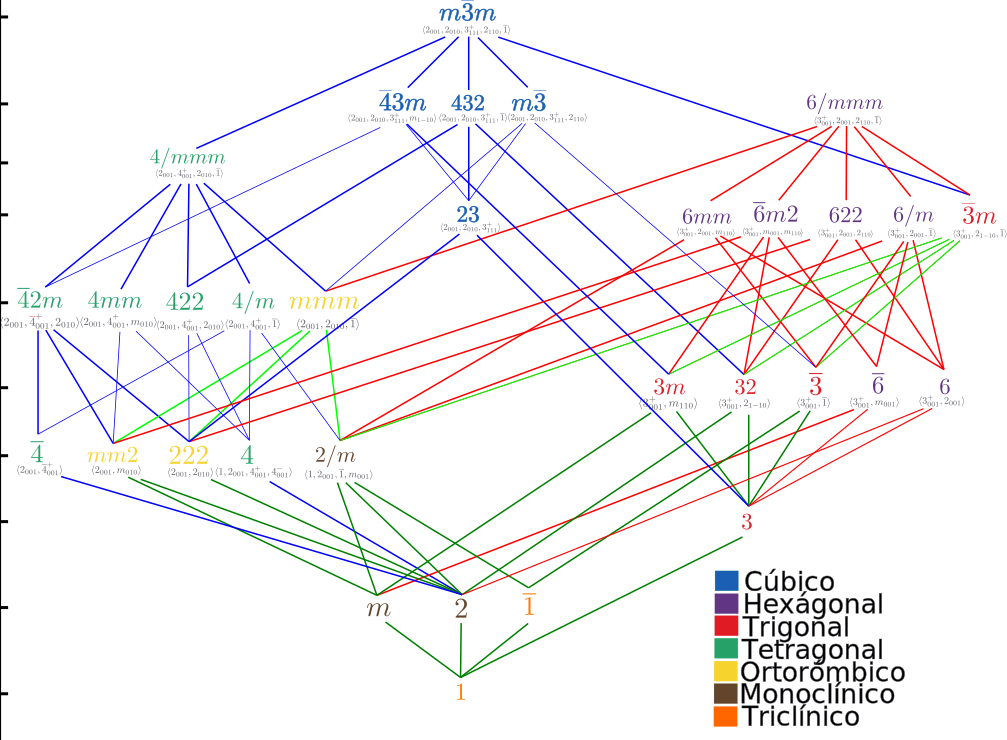
\includegraphics[width=1\textwidth]{matlab/raizatq.png} 
\caption{Relación grupo-subgrupo para los 32 grupos puntuales} 
\label{rai}
\end{figure}


De la unión de $m\overline{3}m$ y $6/mmm$ , $P_{33}$ puede ser una combinación de los 59 elementos\footnote{Ya que el 1 es el elemento identidad y siempre está contenido en el grupo. En total se forman $\sum_{n=1}^{59} (\begin{tabular}{c}
59 \\ 
n \\ 
\end{tabular} )=5.76e+17$ conjuntos, no todos necesariamente tienen estructura de grupo evidentemente. }(los elementos comunes de ambos grupos se presentan en verde): 



\[
\textcolor{blue}{m\overline{3}m} \;\cup\;\textcolor{red}{ 6/mmm}
=\bigl\{
\textcolor{green}{1},\;\textcolor{green}{-1},
\quad
\textcolor{green}{2_{[100]}},\;\textcolor{green}{2_{[010]}},\;\textcolor{green}{2_{[001]}},
\;\textcolor{green}{2_{[110]}},\;\textcolor{green}{2_{[1\bar{1}0]}},
\textcolor{blue}{2_{[101]}},\;\textcolor{blue}{2_{[\bar{1},0,1]}},
\;\textcolor{blue}{2_{[011]}},\;\textcolor{blue}{2_{[0\,1\,\bar{1}]}},
\textcolor{red}{2_{[210]}},\;\textcolor{red}{2_{[120]}}
\]

\[\textcolor{blue}{3^{+}_{[111]}},\;\textcolor{blue}{3^{-}_{[111]}},
\;\textcolor{blue}{3^{+}_{[1\bar{1}\bar{1}]}},\;\textcolor{blue}{3^{-}_{[1\bar{1}\bar{1}]}},
\;\textcolor{blue}{3^{+}_{[\bar{1}1\bar{1}]}},\;\textcolor{blue}{3^{-}_{[\bar{1}1\bar{1}]}},
\;\textcolor{blue}{3^{+}_{[\bar{1}\bar{1}1]}},\;\textcolor{blue}{3^{-}_{[\bar{1}\bar{1}1]}},
\textcolor{red}{3^{+}_{[001]}},\;\textcolor{red}{3^{-}_{[001]}}
\]
 \[\textcolor{blue}{4^{+}_{[100]}},\;\textcolor{blue}{4^{-}_{[100]}},
\;\textcolor{blue}{4^{+}_{[010]}},\;\textcolor{blue}{4^{-}_{[010]}},
\;\textcolor{blue}{4^{+}_{[001]}},\;\textcolor{blue}{4^{-}_{[001]}}\]      
\[\textcolor{red}{6^{+}_{[001]}},\;\textcolor{red}{6^{-}_{[001]}}\]
\[\textcolor{green}{m_{(100)}},\;\textcolor{green}{m_{(010)}},\;\textcolor{green}{m_{(001)}},
\;\textcolor{green}{m_{(110)}},\;\textcolor{green}{m_{(1\bar{1}0)}}\]
%raiz
\[\textcolor{blue}{m_{(101)}},\;\textcolor{blue}{m_{(\bar{1}\,0\,1)}},
\;\textcolor{blue}{m_{(011)}},\;\textcolor{blue}{m_{(0\,1\,\bar{1})}}\quad\]
\[\textcolor{red}{m_{(120)}},\;\textcolor{red}{m_{(210)}}\]
\[\textcolor{blue}{\bar{3}^{+}_{[111]}},\;\textcolor{blue}{\bar{3}^{-}_{[111]}},
\;\textcolor{blue}{\bar{3}^{+}_{[1\bar{1}\bar{1}]}},\;\textcolor{blue}{\bar{3}^{-}_{[1\bar{1}\bar{1}]}},
\;\textcolor{blue}{\bar{3}^{+}_{[\bar{1}1\bar{1}]}},\;\textcolor{blue}{\bar{3}^{-}_{[\bar{1}1\bar{1}]}},
\;\textcolor{blue}{\bar{3}^{+}_{[\bar{1}\bar{1}1]}},\;\textcolor{blue}{\bar{3}^{-}_{[\bar{1}\bar{1}1]}}\]
\[\textcolor{red}{\overline{3}^{+}_{[001]}},\;\textcolor{red}{\overline{3}^{-}_{[001]}}\]
\[\textcolor{blue}{\bar{4}^{+}_{[100]}},\;\textcolor{blue}{\bar{4}^{-}_{[100]}},
\;\textcolor{blue}{\bar{4}^{+}_{[010]}},\;\textcolor{blue}{\bar{4}^{-}_{[010]}},
\;\textcolor{blue}{\bar{4}^{+}_{[001]}},\;\textcolor{blue}{\bar{4}^{-}_{[001]}}\]
\[\textcolor{red}{\overline{6}^{+}_{[001]}},\;\textcolor{red}{\overline{6}^{-}_{[001]}}
\bigr\}=\langle \textcolor{green}{2_{001}},\textcolor{green}{2_{010}},\textcolor{green}{2_{110}},\textcolor{green}{\overline{1}},\textcolor{blue}{3^+_{111}}  \rangle \;\cup \; \langle \textcolor{green}{2_{001}},\textcolor{green}{2_{110}},\textcolor{green}{\overline{1}},\textcolor{red}{3^+_{001}}  \rangle \]





\newpage


Al evaluar los conjuntos que se forman tanto con elementos de ambos conjuntos por separado y como combinación de elementos de ellos se llega al hecho de que \textbf{sí}  se forman nuevos grupos. Sin ir más lejos. veamos esto en los grupos de orden 2. Los ya conocidos de orden 2 son:


\vspace{.2cm}
\[\hspace{-1cm}
\overline{1} = \{ 1, \overline{1} \}
= \{
I, \quad
\begin{pmatrix}
-1 & 0 & 0 \\
0 & -1 & 0 \\
0 & 0 & -1
\end{pmatrix} \}
\qquad
2 = \{ 1, 2_{010} \}
 = \{
I, \quad
\begin{pmatrix}
-1 & 0 & 0 \\
0 & 1 & 0 \\
0 & 0 & -1
\end{pmatrix} \}
\qquad
m = \{ 1, m_{010} \}
= \{
I, \quad
\begin{pmatrix}
1 & 0 & 0 \\
0 & -1 & 0 \\
0 & 0 & 1
\end{pmatrix}  \}
\]


Sin embargo, se pueden formar al menos 17 grupos distintos. Por ejemplo 4 de estos:


\[\hspace{-.5cm}
 \left\{
I,
\begin{pmatrix}
1 & 0 & 0 \\
0 & 1 & 0 \\
0 & 0 & -1
\end{pmatrix}
\right\}
= \{ 1, m_{001} \} \quad 
 \left\{
I,
\begin{pmatrix}
1 & 0 & 0 \\
0 & -1 & 0 \\
0 & 0 & 1
\end{pmatrix}
\right\}
= \{ 1, m_{010} \} \quad 
 \left\{
I,
\begin{pmatrix}
-1 & 0 & 0 \\
0 & 1 & 0 \\
0 & 0 & 1
\end{pmatrix}
\right\}
= \{ 1, m_{100} \} \quad 
\left\{
I,
\begin{pmatrix}
0 & 1 & 0 \\
1 & 0 & 0 \\
0 & 0 & -1
\end{pmatrix}
\right\}
= \{ 1, 2_{110} \} 
\]



Nos podemos convencer de esto notando que la condición de grupo, para conjuntos de dos matrices, es de hecho bastante laxa. Basta con que la matriz que no es la identidad sea su propio elemento inverso. \\

\vspace{.2cm}

Vemos por tanto que si existen nuevos grupos diferentes (aún pudiendo pertenecer a la misma clase de conjugación)  a los 32 ya conocidos, con perfecto sentido. Ya que los elementos que los componen son operaciones de simetría válidas. \\
\vspace{.2cm}

 Por tanto llegamos a una contradicción, $P_{33}$ es cristalográfico $\wedge$ ($P_{33}\notin \mathcal{P} = \{ P_1, P_2, \ldots, P_{32} \}\;\leftrightarrow \; P_{33}
$ no es cristalográfico). Por tanto $P_{33}$ no es cristalográfico. Solo cabe decir que un grupo es cristalográfico si es uno de los 32, aún habiendo más grupos puntuales que contienen operaciones de grupos cristálográficos y que por tanto satisfacen las condiciones de periodicidad de una red.



\section{Grupos espaciales cristalográficos}



Una operación de grupo espacial cristalográfico es una isometría que mapea un patrón cristalino sobre sí mismo. Dado que las isometrías son invertibles y la composición de dos isometrías deja el patrón cristalino invariante como un todo si las dos isometrías individuales lo hacen, las operaciones de grupo espacial forman un grupo $\mathcal{G}$, llamado un \textit{grupo espacial cristalográfico}.\\
 
 \vspace{.2cm}

Una operación de grupo espacial se compone de una transformación lineal del espacio vectorial subyacente y una traslación. Una vez que se ha elegido un sistema de coordenadas, las operaciones de grupo espacial se representan convenientemente como pares matriz–columna $(W, \mathbf{w})$, donde $W$ es la parte lineal y $\mathbf{w}$ la \textit{parte de traslación}, y un punto con coordenadas $\mathbf{x}$ se mapea a $W\mathbf{x} + \mathbf{w}$ .\\
 \vspace{.2cm}
Una traslación es un par matriz–columna de la forma $(I, \mathbf{w})$, donde $I$ es la matriz unidad y todas las traslaciones tomadas juntas forman el subgrupo de traslación $\mathcal{T}$ de $\mathcal{G}$. El subgrupo de traslación es un grupo infinito que forma un subgrupo  de $\mathcal{G}$. El grupo cociente $\mathcal{G}/\mathcal{T}$ es un grupo finito que es isomorfo con el grupo de partes lineales de $\mathcal{G}$ vía la aplicación $(W, \mathbf{w}) \mapsto W$, que simplemente omite la parte de traslación. Estos grupos que contienen las partes lineales $\mathcal{P}=\{\textbf{W}\; \vert \; (\textbf{W},\textbf{w})\in \mathcal{G}\}$ son los grupos puntuales cristalográficos ya analizados en la sección anterior  .



\subsection{Red cristalina}




En este sentido cabe representar un patrón cristalino con el concepto matemático de red. Un conjunto de puntos $X\in \mathbb{R}^3$, es un cristal si  y solo si L es discreto y sym(L)\footnote{$\mathrm{sym}(X)$ denota el grupo de isometrías del espacio euclidiano que dejan $X$ invariante.} es grupo espacial cristalográfico. Más concreto, dada la base $\mathbb{B}=\{\textbf{a},\textbf{b},\textbf{c},\quad \vert \quad \textbf{a},\textbf{b},\textbf{c}\in \mathbb{R}^3 \} $, se define una red L como el conjunto de puntos tal les que:


\vspace{.1cm}
\[L=\{\;(l,m,n)_\mathbb{B}\quad \vert  \quad l,m,n \in \mathbb{Z} \}\]

\vspace{.1cm}


Los vectores de traslación de un patrón cristalino forman una red con base de red $\mathbf{a}, \mathbf{b}, \mathbf{c}$ en el sentido de la definición anterior. Por definición, una red está determinada por una base de red. Sin embargo, obsérvese que toda red  tridimensional o bidimensional  tiene infinitas bases.\\
\vspace{.2cm}


Una red \( \mathbf{L} \) puede utilizarse para subdividir \( \mathbb{R}^3 \) en celdas de volumen finito que todas tengan la misma forma. La idea es definir un subconjunto adecuado \( \mathbf{C} \) de \( \mathbb{R}^3 \) tal que los traslados de \( \mathbf{C} \) mediante los vectores en \( \mathbf{L} \) cubran \( \mathbb{R}^3 \) sin superponerse. Tal subconjunto \( \mathbf{C} \) se denomina celda unidad de \( \mathbf{L} \):



    \[
    \mathbf{C} = \{\; (x,y,z)_\mathbb{B} \quad  \mid \quad  0 \leq x, y, z < 1 \; \}
    \]


En este sentido, el grupo puntual  describe las simetrías de la celda unitaria que se mantienen cuando se ignoran las traslaciones.
\newpage
\textit{Ejemplo:}























\newpage
\begin{thebibliography}{9}

\bibitem{gonzalez2014} 
Artemio González López. 
\textit{Simetrías y Grupos en Física: Notas de curso}. 
Madrid, enero de 2014.

\bibitem{itc}
Mois I. Aroyo (Ed.). 
\textit{International Tables for Crystallography, Volume A: Space-Group Symmetry}. 
Sixth Edition, Wiley, 2014.

\bibitem{bilbao}
Bilbao Crystallographic Server.  
Disponible en: \texttt{https://www.cryst.ehu.es}.

\bibitem{gallian}
Joseph A. Gallian.  
\textit{Contemporary Abstract Algebra}.  
Ninth Edition, Cengage Learning, 2017.

\bibitem{giacovazzo}
C. Giacovazzo (Ed.).  
\textit{Fundamentals of Crystallography}.  
Oxford University Press, 2002.



\end{thebibliography}

















\end{document}
